\documentclass[fleqn]{article}
\usepackage[spanish]{babel}
\renewcommand\spanishtablename{Tabla}
\usepackage{amsmath}
\usepackage{amsthm}
\usepackage{blkarray}
\usepackage{graphicx}
\graphicspath{{figs/}}
\usepackage[utf8]{inputenc}

%%%%%%%% MARGIN
\usepackage[left=1in, right=1in, top=0.8in, bottom=0.8in]{geometry}

%%%%%%%% NO PARAGRAPH INDENT
% https://tex.stackexchange.com/questions/27802/set-noindent-for-entire-file
\setlength\parindent{0pt}

%%%%%%%% SUB-FIGURE PACKAGE
\usepackage{subcaption}

\usepackage{pdfpages}

%%%%%%%% HYPERREF PACKAGE
\usepackage{hyperref}
\hypersetup{linkcolor=blue}
\hypersetup{citecolor=blue}
\hypersetup{urlcolor=blue}
\hypersetup{colorlinks=true}

%%%%%%%% MULTI-COLUMNS PACKAGE
\usepackage{multicol}

%%%%%%%% SETS DEFINITIONS
\usepackage{amssymb}
%%%% Important sets
\renewcommand{\O}{\mathbb{O}}
\newcommand{\N}{\mathbb{N}}
\newcommand{\Z}{{\mathbb{Z}}}
\newcommand{\Q}{{\mathbb{Q}}}
\newcommand{\R}{{\mathbb{R}}}
\newcommand{\norm}[1]{\left\lVert#1\right\rVert}
%%%% Statistics
\newcommand{\E}[1]{\mathbb{E}\left[#1 \right]}
\newcommand{\V}[1]{\mathrm{Var}\left[#1 \right]}


%%%% Superscript to the left
% https://latex.org/forum/viewtopic.php?t=455
\usepackage{tensor}
\newcommand{\app}[3]{\tensor*[^{#1}]{\left(#2, #3\right)}{}}


%%%%%%%% SPLIT EQUATIONS
% https://tex.stackexchange.com/questions/51682/is-it-possible-to-pagebreak-aligned-equations
\allowdisplaybreaks

%%%%%%%% CODE RENDERING
% Compile with flag -shell-escape
\usepackage{minted}

%%%%%%%% EXAM PACKAGE
\usepackage{mathexam}

%%%%%%%% CHANGE MARGINS ITEMIZE
\usepackage{enumitem}

%%%%%%%% START DOCUMENT

\ExamClass{ESTADÍSTICA NO PARAMÉTRICA}
\ExamName{EXAMEN FINAL}
\ExamHead{\today}

\let\ds\displaystyle

\begin{document}
 \vspace{0.3cm}
   % Information of the student
   \begin{itemize}[leftmargin=6.25cm, labelsep=0.5cm]

     \item[\textit{Nombre}] \scalebox{1.2}{David Plazas Escudero} % Name
     \item[\textit{Código}] 201710005101 % Code

   \end{itemize}
\vspace{0.3cm}
El código para dar respuestas a las preguntas de este examen puede encontrarse \href{https://github.com/Daples/daples/blob/master/nps/code-exam.ipynb}{aquí.}
\section*{1. a)}
\textbf{Enunciado:} \textit{Grafique en un mismo plano las funciones de distribución empíricas de los tiempos de vida de los 13 años. Explique con base en las gráficas de las funciones, si es observable un efecto de mejoría en los tiempos de vida a través del tiempo. Interprete los intervalos donde la función del primer año es mayor a la del último.}\\
\textbf{Solución:} La gráfica de las distribuciones empíricas (ECDFs) para los tiempos de vida de los 991 dispositivos, durante 13 años, se muestra en la Figura \ref{fig:1a}. En esta figura se puede observar que efectivamente hay una mejoría en los tiempos de vida de los dispositivos. Es claro la ECDF de los años más recientes está siempre por debajo de los primeros años; esto implica que hay un mayor chance de que los dispositivos recientes tengan mayor tiempo de vida. Sea $X$ el tiempo de vida de un dispositivo del año más reciente y $Y$ del año más antiguo, se sigue que $\hat{F}_X(t)\leq\hat{F}_Y(t)$, luego se puede afirmar que $X$ es mejor a $Y$.
\begin{figure}[H]
    \centering
    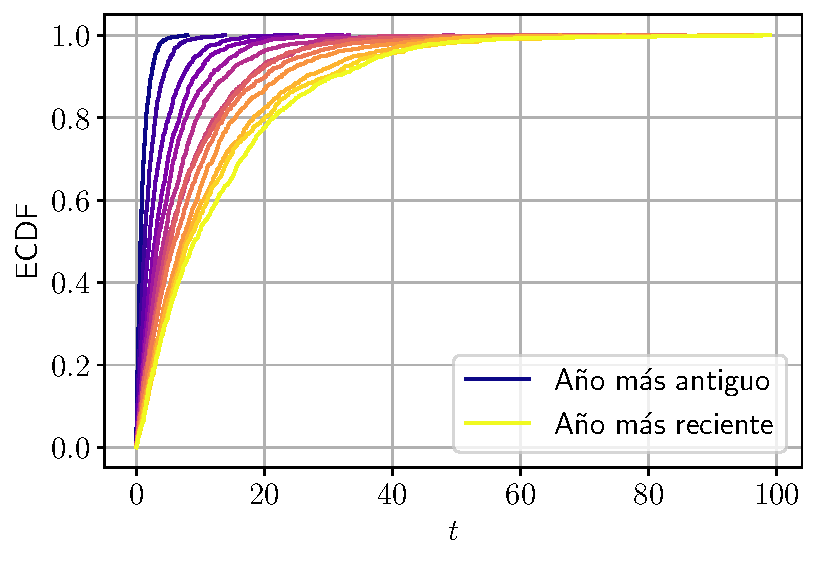
\includegraphics[scale=.6]{1a.pdf}
    \caption{ECDFs de tiempos de vida.}
    \label{fig:1a}
\end{figure}

\section*{1. b)}
\textbf{Enunciado:} \textit{Calcule y grafique las bandas de confianza a un 90\% de confianza para la función de distribución empírica del primer año.}\\
\textbf{Solución:} Las bandas de confianza utilizadas están basadas en la desigualdad de Dvoretzky-Kiefer-Wolfowitz (ver \cite[p. 14]{wasserman2006}). Las bandas se presentan en la Figura \ref{fig:1b}.
\begin{figure}[H]
    \centering
    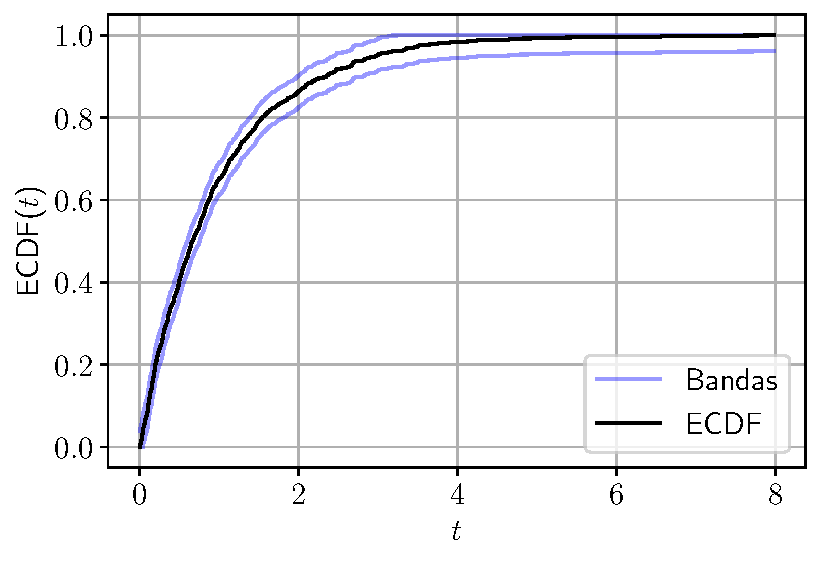
\includegraphics[scale=.6]{1b.pdf}
    \caption{Bandas de confianza para la ECDF del primer año con $\alpha=0.10$.}
    \label{fig:1b}
\end{figure}

\section*{1. c)}
\textbf{Enunciado:} \textit{Grafique en un mismo plano la distribución empírica del último año y la distribución teórica de una exponencial con media 13. ¿Considera usted que hay un buen ajuste? Haga lo mismo con las densidad estimada y la teórica. Determine computacionalmente si se cumple en este par de distribuciones el Teorema de Glivenko-Cantelli.}\\
\textbf{Solución:} Primero, se muestra la gráfica de la densidad de la distribución exponencial y la densidad estimada a partir de los datos, en la Figura \ref{fig:1c1}. Esta estimación se realizó utilizando el kernel de Epanechnikov con un ancho de banda de 2.

\begin{figure}[H]
    \centering
    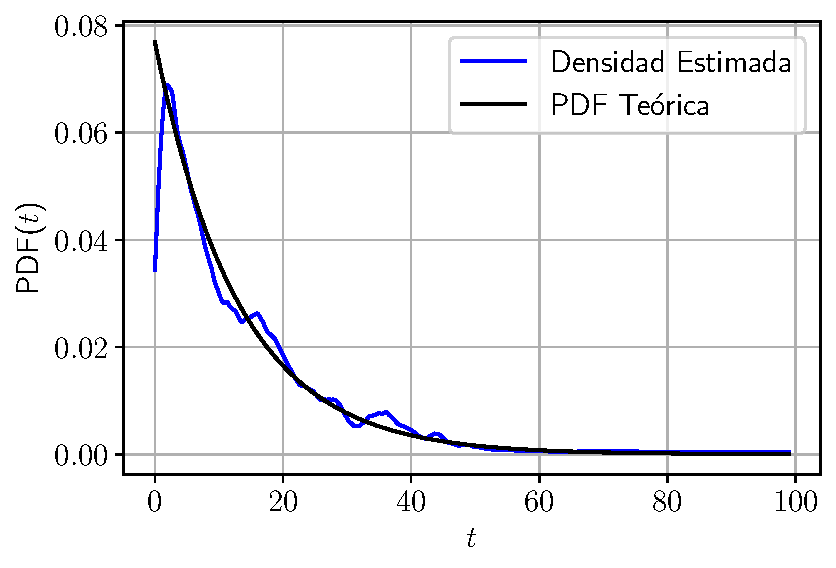
\includegraphics[scale=.6]{1c_2.pdf}
    \caption{Estimación vs. teórica para la densidad.}
    \label{fig:1c1}
\end{figure}

Adicionalmente, la gráfica de la ECDF y la distribución exponencial se muestra en la Figura \ref{fig:1c2}.

\begin{figure}[H]
    \centering
    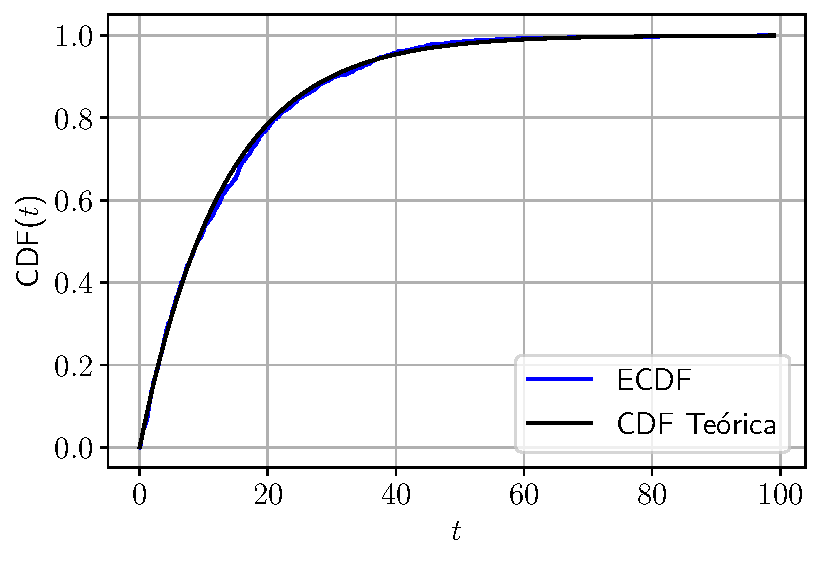
\includegraphics[scale=.6]{1c_1.pdf}
    \caption{Estimación vs. teórica para la acumulada.}
    \label{fig:1c2}
\end{figure}
Claramente se observa que ambas distribuciones de ajustan casi perfectamente, lo que muestra buena evidencia de que se cumple el teorema de Glivenko-Cantelli. Este teorema afirma que el supremo de la diferencia entre la distribución empírica y la real converge casi seguramente a 0 cuando el tamaño de la muestra se aumenta \cite[p. 14]{wasserman2006}. Para evidenciar este efecto de una mejor manera, en la Figura \ref{fig:1c3} se presenta los supremos de estas diferencias para diferentes tamaños de muestra. Claramente se evidencia que este supremo disminuye a medida que se aumenta el tamaño de la muestra para la ECDF.
\begin{figure}[H]
    \centering
    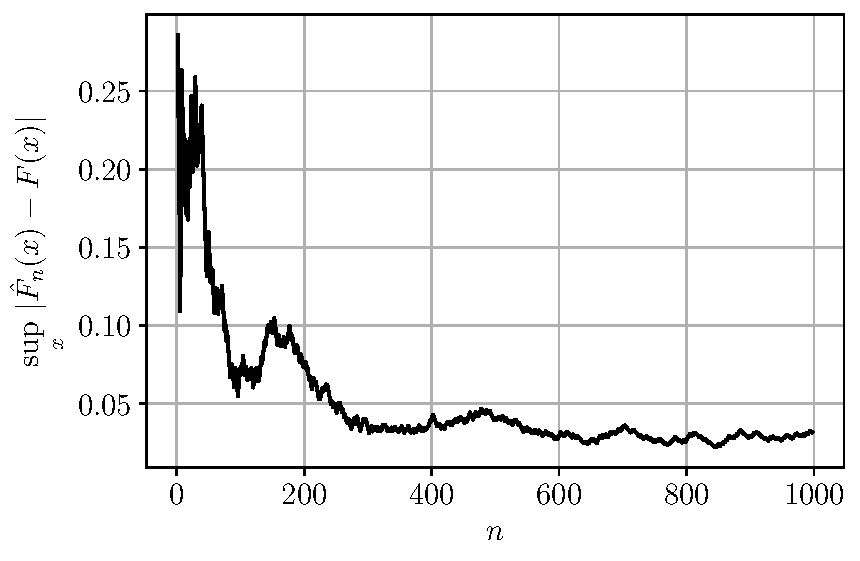
\includegraphics[scale=.6]{1c_3.pdf}
    \caption{Supremo de las diferencias para diferentes tamaños de muestra.}
    \label{fig:1c3}
\end{figure}
\section*{1. d)}
\textbf{Enunciado:} \textit{Considere $X_1,X_2,\hdots$ una sucesión de variables aleatorias. Pruebe que $\{X_n\}_{n\in\mathbb{N}}$ converge en probabilidad a $b$ si 
\[
\lim_{n\rightarrow\infty}E(X_n)=b \ y \ \lim_{n\rightarrow\infty}V(X_n)=0
\]}\\
\textbf{Solución:} Sea $\{X_n\}_{n\in\mathbb{N}}$ una sucesion de variables aleatorias que satisfacen que 
\begin{equation}\label{eq:cond}
\lim_{n\rightarrow\infty}E(X_n)=b \ y \ \lim_{n\rightarrow\infty}V(X_n)=0.
\end{equation}

Se puede ver que la convergencia en probabilidad está implicada por la convergencia en error cuadrático medio (MSE). Recordemos que una sucesión $\{Y_n\}_{n\in\mathbb{N}}$ converge en MSE a una variable aleatoria $Y$ si satisface
\[
  \lim_{n\rightarrow\infty}E\left[(Y_n-Y)^2\right]=0.
\]

Adicionalmente se sabe que $E\left[(Y_n-Y)^2\right]=V(Y_n)+\mathrm{Bias}^2(Y_n,Y)$. Calculemos el sesgo para nuestro caso de $Y_n=X_n$ y $Y=X=b$:
\begin{align*}
    \mathrm{Bias}^2(X_n,X) = \left[E(X_n) - b\right]^2=E^2(X_n) - 2bE(X_n) + b^2.
\end{align*}
Luego,
\begin{align*}
    E\left[(X_n-X)^2\right]=V(X_n)+E^2(X_n) - 2bE(X_n) + b^2
\end{align*}
tomando límite a ambas partes se tiene
\begin{align*}
    \lim_{n\rightarrow\infty}E\left[(X_n-X)^2\right]=&\lim_{n\rightarrow\infty}\left[V(X_n)+E^2(X_n) - 2bE(X_n) + b^2\right]\\
    =&\lim_{n\rightarrow\infty}V(X_n)+\lim_{n\rightarrow\infty}E^2(X_n) - 2b\lim_{n\rightarrow\infty}E(X_n) + b^2\\
    =&0+b^2-2b^2+b^2=0
\end{align*}
Luego, $\{X_n\}_{n\in\mathbb{N}}$ converge en MSE, y por lo tanto en probabilidad, a $b$.
 
\section*{1. e)}
\textbf{Enunciado:} \textit{Considere los tiempos de vida del primer año. Calcule un intervalo de confianza bootstrap para el tiempo de vida máximo. Calcule el sesgo de $T_{[n]}$ y la varianza por el método de Jackknife.}

\textbf{Solución:} Los intervalos de confianza (CI) se muestran en la Tabla \ref{tab:cis}, estos CI fueron construidos en una remuestreo Bootstrap de 10000 muestras con repetición. El sesgo obtenido por Jackknife es $b_{\mathrm{jack}}=-0.66$ y la varianza estimada es $v_{\mathrm{jack}}=4.34$.
\begin{table}[H]
\centering
\begin{tabular}{ll}
\hline
\multicolumn{1}{c}{\textbf{Método}} & \textbf{Ci} \\ \hline
Normal                              & (6.91, 9.06)  \\
Percentile                          & (7.98, 9.41)  \\
Studentized                         & (7.98, 12.49) \\
Pivotal                             & (7.98, 9.41)  \\ \hline
\end{tabular}
\caption{Intervalos de confianza Bootstrap para el máximo.}
\label{tab:cis}
\end{table}
\section*{1. f)}
\textbf{Enunciado:} \textit{La variable costos es el costo en dólares de reparacióon de los dispositivos observados en el primer año. Realice una regresión para intentar explicar el costo de reparación en términos del tiempo de duración del dispositivo.}

\textbf{Solución:} 
La gráfica de dispersión se presenta en la Figure \ref{fig:1f1}. 
\begin{figure}[H]
    \centering
    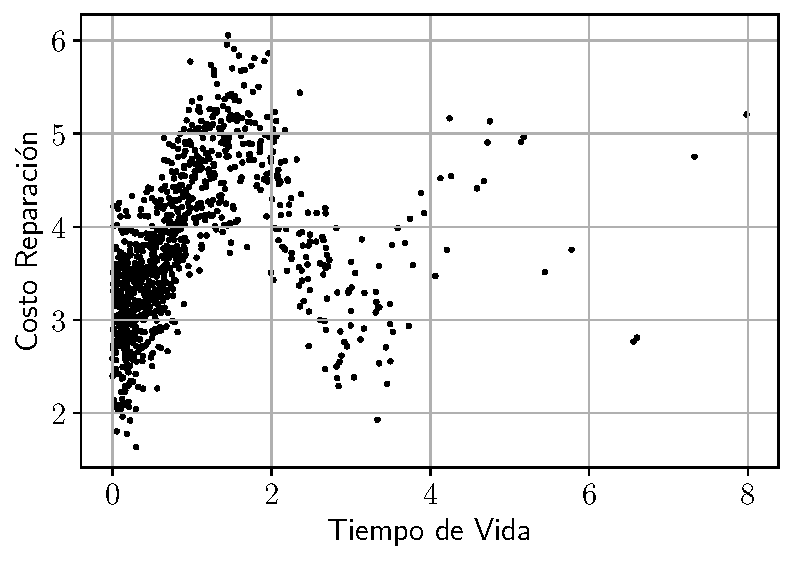
\includegraphics[scale=.6]{1f_scatter.pdf}
    \caption{Gráfico de dispersión de costos contra tiempo de vida.}
    \label{fig:1f1}
\end{figure}
Es claro que los datos no siguen una tendencia lineal, pero como en este ejercicio no se especifica qué tipo de regresión, se intentará primero con una regresión lineal basada en mínimos cuadrados ordinarios (OLS). El resultado se presenta en la Figura \ref{fig:1f2} y se observa que es un modelo deplorable. 
\begin{figure}[H]
    \centering
    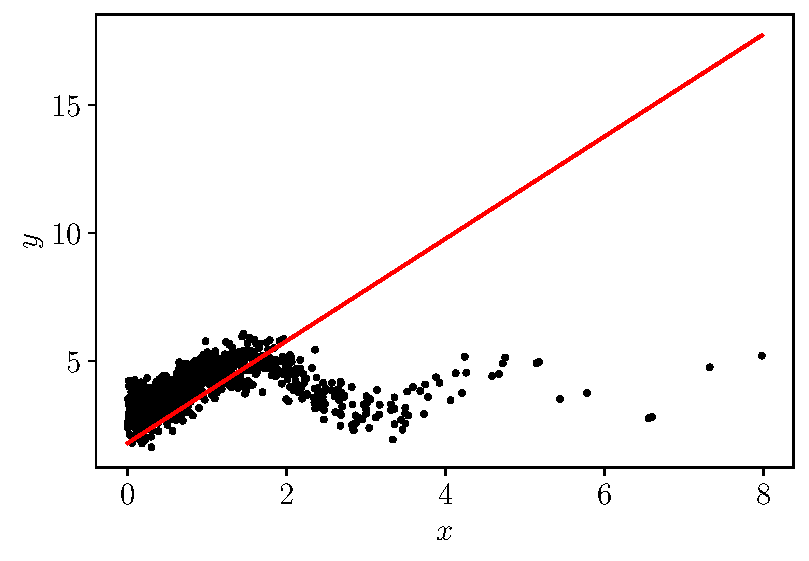
\includegraphics[scale=.6]{1f.pdf}
    \caption{Regresión por OLS.}
    \label{fig:1f2}
\end{figure}

Alternativamente, se intentará una regresión por kernels de tipo Nadaraya–Watson. La regresión de hizo utilizando el kernel de Epanechnikov con ancho de banda de $0.5$ y se pueden observar los resultados en la Figura \ref{fig:1f3}. Esta regresión claramente se ajusta mejor a los datos obtenidos, logrando capturar la tendencia sinusoidal presente.
\begin{figure}[H]
    \centering
    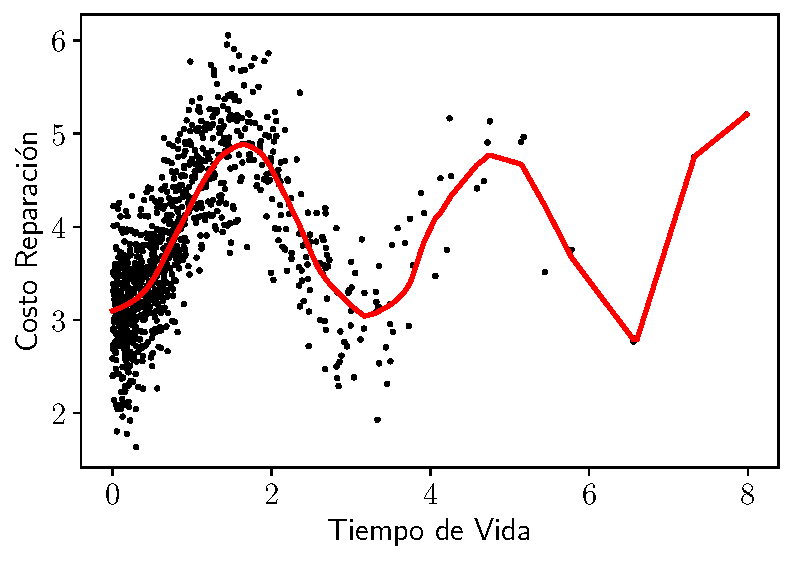
\includegraphics[scale=.6]{1f_nw.pdf}
    \caption{Regresión por Nadaraya-Watson.}
    \label{fig:1f3}
\end{figure}

\section*{1. g)}
\textbf{Enunciado:} \textit{Pase un test de rangos para identificar qué años tuvieron una duración en el dispositivo con diferente distribución. ¿Qué conclusión se obtiene?.}

\textbf{Solución:} Para este apartado de realizó un test ``ranksum'' para cada par de años, confeccionando la matriz presentada a continuación, donde un 0 en la  posición $(i,j)$ indica hay evidencia suficiente para afirmar que el año $i$ y el $j$ provienen de la misma distribución. El 1 indica el caso contrario. Este test se realizó con $\alpha=0.05$. Esta matriz nos indica que prácticamente todos los años provienen de distintas distribuciones, con algunas excepciones de años consecutivos.

\begin{table}[H]
\centering
\begin{tabular}{c|ccccccccccccc}
\textbf{}   & \textbf{1} & \textbf{2} & \textbf{3} & \textbf{4} & \textbf{5} & \textbf{6} & \textbf{7} & \textbf{8} & \textbf{9} & \textbf{10} & \textbf{11} & \textbf{12} & \textbf{13} \\ \hline
\textbf{1}  & 0          & 1          & 1          & 1          & 1          & 1          & 1          & 1          & 1          & 1           & 1           & 1           & 1           \\
\textbf{2}  & 1          & 0          & 1          & 1          & 1          & 1          & 1          & 1          & 1          & 1           & 1           & 1           & 1           \\
\textbf{3}  & 1          & 1          & 0          & 1          & 1          & 1          & 1          & 1          & 1          & 1           & 1           & 1           & 1           \\
\textbf{4}  & 1          & 1          & 1          & 0          & 1          & 1          & 1          & 1          & 1          & 1           & 1           & 1           & 1           \\
\textbf{5}  & 1          & 1          & 1          & 1          & 0          & 1          & 1          & 1          & 1          & 1           & 1           & 1           & 1           \\
\textbf{6}  & 1          & 1          & 1          & 1          & 1          & 0          & 1          & 1          & 1          & 1           & 1           & 1           & 1           \\
\textbf{7}  & 1          & 1          & 1          & 1          & 1          & 1          & 0          & 0          & 1          & 1           & 1           & 1           & 1           \\
\textbf{8}  & 1          & 1          & 1          & 1          & 1          & 1          & 0          & 0          & 1          & 1           & 1           & 1           & 1           \\
\textbf{9}  & 1          & 1          & 1          & 1          & 1          & 1          & 1          & 1          & 0          & 1           & 1           & 1           & 1           \\
\textbf{10} & 1          & 1          & 1          & 1          & 1          & 1          & 1          & 1          & 1          & 0           & 1           & 1           & 1           \\
\textbf{11} & 1          & 1          & 1          & 1          & 1          & 1          & 1          & 1          & 1          & 1           & 0           & 0           & 1           \\
\textbf{12} & 1          & 1          & 1          & 1          & 1          & 1          & 1          & 1          & 1          & 1           & 0           & 0           & 0           \\
\textbf{13} & 1          & 1          & 1          & 1          & 1          & 1          & 1          & 1          & 1          & 1           & 1           & 0           & 0          
\end{tabular}
\end{table}


\section*{1. h)}
\textbf{Enunciado:} \textit{Pase un test de homogeneidad multivariante para identificar si los primeros 400 registros vienen de la misma distribución de los últimos 400. Con el mismo test, verifique si los 5 primeros años vienen de la misma distribución de los 5 últimos. ¿Qué conclusión se puede sacar de acuerdo al resultados de los test.}

\textbf{Solución:} El test de homogeneidad se realizó siguiendo la metodología expuesta en clase. A continuación se hará una breve descripción del proceso:
\begin{enumerate}
    \item Se tienen dos poblaciones $X\in\mathbb{R}^{n\times p}$ y $Y\in\mathbb{R}^{m\times p}$ $p$-variadas. Se construye una nueva población $Z\in\mathbb{R}^{(n+m)\times p}$ como la concatenación de $X$ con $Y$.
    \item Para cada $z\in Z$, se calcula la profundidad estadística (Tukey o Mahalanobis) respecto a la masa de datos de $X$, construyendo el vector de profundidades $Z_X\in\mathbb{R}^{(n+m)}$. De la misma manera se construye $Z_Y\in\mathbb{R}^{(n+m)}$.
    \item Se construye una regresión OLS sobre $(Z_X,Z_Y)$. La gráfica de dispersión de $(Z_X,Z_Y)$ es conocida como el D-D plot.
    \item Si $\beta_1=1$ y $\beta_0=0$, se tendrá perfecta dependencia lineal $Z_X=Z_Y$ y se concluirá que los datos provienen de la misma distribución.
\end{enumerate}
La implementación considerada para este punto utiliza la profunidad de Tukey, con 500 direcciones aleatorias. Para la primera parte, se tomaron los primeros y últimos 400 registros. Es claro que se esperaría que estos datos provengan de la misma distribución. El gráfico de dispersión de $(Z_X,Z_Y)$ y la regresión se muestran en la Figura \ref{fig:1h1}. Los resultados del modelo de regresión son: $\beta_1=0.972$ y $\beta_0=0.002$. Con lo que se puede concluir que las dos muestras son tomadas de la misma población.

\begin{figure}[H]
    \centering
    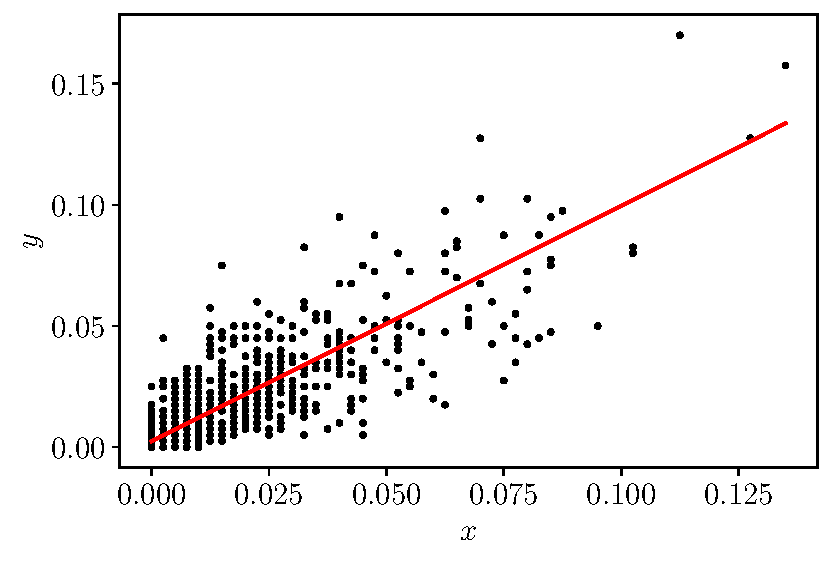
\includegraphics[scale=.6]{1h_1.pdf}
    \caption{D-D plot para los primeros y últimos 400 registros.}
    \label{fig:1h1}
\end{figure}

Para la segunda parte, la primera población corresponde a los primeros 5 años de registros, y la segunda a los últimos 5. En este caso, se espera que las poblaciones no vengan de la misma distribución, debido a que, como se explicó en el punto 1.a), los tiempos de vida de los primeros años son menores a los de los años más recientes. La Figura \ref{fig:1h2} muestra los resultados de la dispersión y la regresión ajustada. En este caso, no era necesario hacer el modelo de regresión, pues es evidente que los datos nunca podrían ajustarse a la recta identidad.

\begin{figure}[H]
    \centering
    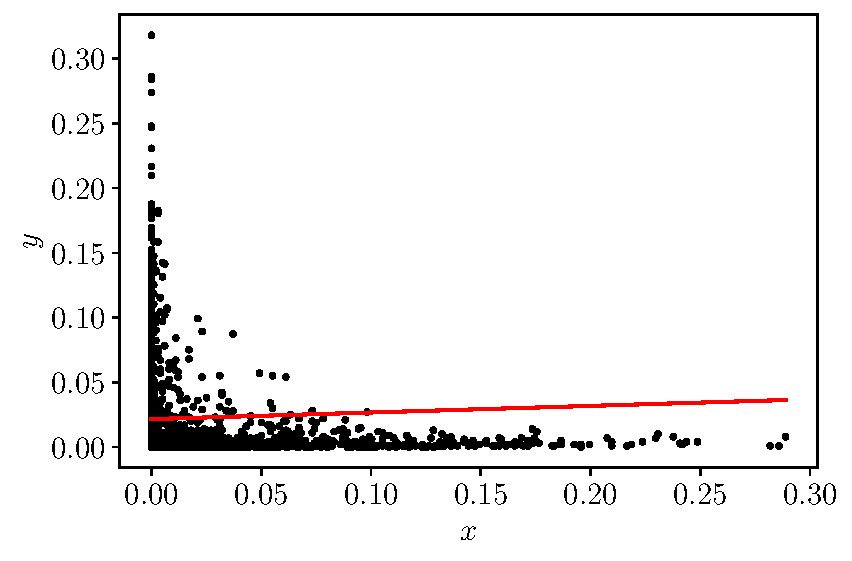
\includegraphics[scale=.6]{1h_2.pdf}
    \caption{D-D plot para los primeros y últimos 5 años.}
    \label{fig:1h2}
\end{figure}

\section*{1. i)}
\textbf{Enunciado:} \textit{ Considere $\beta = [13, 12, 11,\hdots, 3, 2, 1]$. Suponga que $y=vida\times \beta^T + \xi$, Donde $\xi$ es un ruido normal de media cero y desviación 50. Realice con varios modelos de regresión lineal no paramétrica y robusta, modificando la matriz de covarianzas por una versión robusta o no paramétrica o combinación de ellas (Kendall, Spearman, fastMCD, máxima kurtosis, shrinkages) para identificar cuál de ellas tiene mejor desempeño. Incluya la regresión por mínimos cuadrados para comparación.}


\textbf{Solución:} Los métodos de regresión robusta están basados en que los $\beta$ del modelo de regresión pueden ser escritos como $\hat{\beta}=\Sigma_{xx}^{-1}\Sigma_{xy}$, donde se cambia la estimación usual de las covarianzas por estimadores más robustos. En este caso se utilizará la matriz de comedianas, la estimación basada en las correlaciones de Kendall y Spearman, los métodos de fast MCD y shrinkages disponibles en el paquete \texttt{sklearn} de \texttt{Python}. Finalmente estas regresiones serán comparadas con la estimación usual por mínimos cuadrados ordinarios (OLS). Como no se puede observar directamente la regresión, debido a que se trabaja en el hiperplano 13-dimensional, se evaluará el performance de cada regresión tomando la norma usual de la diferencia entre el vector de betas estimado $\hat{\beta}$ y el vector real de $\beta$. Los resultados se presentan en la Tabla \ref{tab:meth}. Esta tabla muestra que el mejor desempeño fue obtenido por la regresión OLS y el de peor fue el de Fast MCD.

\begin{table}[H]
\centering
\begin{tabular}{cc}
\hline
\textbf{Método} & \textbf{$||\hat{\beta}-\beta^T||_2$} \\ \hline
OLS             & 1.429                                           \\
Spearman        & 3.471                                           \\
Comedian        & 6.186                                           \\
Shrinkages      & 10.080                                          \\
Kendall         & 11.147                                          \\
Fast MCD        & 21.002                                          \\ \hline
\end{tabular}
\caption{Comparación entre los métodos para la regresión.}
\label{tab:meth}
\end{table}


\bibliographystyle{plain}
\bibliography{refs}
\end{document}
